\documentclass{article}               % paper=a4,bibliography=totoc,numbers=noenddot,fontsize=11pt
\usepackage[a4paper, left=2cm, right=2cm, top=2cm]{geometry}
\usepackage[inline]{enumitem}
\usepackage[german]{babel}
\usepackage[T1]{fontenc}
\usepackage[latin1, utf8]{inputenc}
\usepackage{graphicx}
\usepackage{amsmath,amssymb,amstext}
% \usepackage{ulem}   % underline: https://www.namsu.de/Extra/pakete/Ulem.html
\usepackage{verbatim}   % no translation of Latex-Code: http://www.weinelt.de/latex/verbatim.html 
\usepackage{placeins}   % FloatBarrier to separate Sections: https://golatex.de/wiki/placeins  
% \usepackage{xcolor,import}  % colored boxes: https://www.namsu.de/Extra/pakete/Xcolor.html 
\usepackage{csquotes}   % correct quoting: https://tex.stackexchange.com/questions/39285/whats-the-advantage-of-using-csquotes-over-using-an-editors-auto-replacement-f  
\usepackage{nicefrac}   % \nicefrac{a}{b} >>> a/b
\usepackage{icomma}
\usepackage[format=plain]{caption}
% \usepackage{svg}
\usepackage{subcaption}
\usepackage{mathtools}
\usepackage{float}
\usepackage{wrapfig}
\usepackage[pdfborder={0 0 0}]{hyperref}
\usepackage{caption}
\usepackage[export]{adjustbox}
\usepackage{mathrsfs}
\usepackage{bm}
\usepackage{multirow}
\usepackage{booktabs}
\usepackage{siunitx}
\usepackage[table]{xcolor}
\usepackage[style=numeric-comp, natbib, backend=biber, backref=true, sorting=none, maxbibnames=99]{biblatex}
% \DeclareFieldFormat
%   [article,inbook,incollection,inproceedings,patent,thesis,
%    unpublished,techreport,misc,book]
%   {title}{\mkbibquote{#1}}
% \DeclareFieldFormat{apacase}{#1}
% \DeclareLanguageMapping{american}{american-apa}

\newcounter{myitemcounter}

\newcommand{\myitemlabel}{$\bullet$\ }

\newcommand{\myitem}{%
\stepcounter{myitemcounter}
\myitemlabel
}

\newcommand{\anitem}[1]{%
\myitem #1 &
}

\newcommand{\lastitem}[1]{%
\myitem #1 \\
}

\newenvironment{inlineitemize}
{\setcounter{myitemcounter}{0}
\begin{center} 
\begin{tabular}{llll} % you won't want more columns
}
{\end{tabular}
\end{center}}

\newenvironment{inlineenumerate}
{\setcounter{myitemcounter}{0}
\renewcommand{\myitemlabel}{(\alph{myitemcounter})\ }
\begin{tabular}{lllllllllll}
}
{\end{tabular}}


\ExecuteBibliographyOptions{doi=false}
\ExecuteBibliographyOptions{doi=false}
\DeclareFieldFormat{doilink}{%
\iffieldundef{doi}{#1}%
{\href{\thefield{doi}}{#1}}}

\DeclareBibliographyDriver{article}{%
  \usebibmacro{bibindex}%
  \usebibmacro{begentry}%
  \usebibmacro{author/translator+others}%
  \setunit{\labelnamepunct}\newblock
  \usebibmacro{title}%
  \newunit
  \printlist{language}%
  \newunit\newblock
  \usebibmacro{byauthor}%
  \newunit\newblock
  \usebibmacro{bytranslator+others}%
  \newunit\newblock
  \printfield{version}%
  \newunit\newblock
  \usebibmacro{in:}%
  \printtext[doilink]{%
  \usebibmacro{journal+issuetitle}%
  \newunit
  \usebibmacro{byeditor+others}%
  \newunit
  \usebibmacro{note+pages}%
  }%
  \newunit\newblock
  \iftoggle{bbx:isbn}
    {\printfield{issn}}
    {}%
  \newunit\newblock
  \usebibmacro{doi+eprint+url}%
  \newunit\newblock
  \usebibmacro{addendum+pubstate}%
  \setunit{\bibpagerefpunct}\newblock
  \usebibmacro{pageref}%
  \usebibmacro{finentry}}

\graphicspath{{../Bilder}}
\bibliography{EinzelSpek}
\DeclareUnicodeCharacter{2212}{-}
\begin{document}
  \setlength{\parindent}{0em}
    \begin{titlepage}
        \centering
        
\includegraphics[width=11cm,height=3.5cm,angle=0]{LogoUniBayreuth.png}
        \vspace{0.5cm}
        {\large \textbf{\\Universität Bayreuth\\Physikalisches Institut\\Physikalisches Praktikum PPD}\\}
        \vspace{2.5cm}
        {\Huge \textbf{Einzelmolekülspektroskopie}\\}
        \vspace{2.5cm}
        {\LARGE \textbf{Ausarbeitung - Gruppe 1}\\}
        \vspace{0.5cm}
        {\large \textbf{von}\\}
        {\LARGE \textbf{Max Gießübel}\\}
        {\LARGE \textbf{Toni Zimmermann}\\} 	
        \vspace{2cm}
        {\large \textbf{Versuchstermin: 29.02.2024}\\}
        {\large \textbf{Abgabetermin: 08.03.2024}\\}
        \vspace{2cm}
        {\large \textbf{Betreuer\\}}
        {\LARGE \textbf{Dr.~Uwe Gerken\\}}
        \vfill
    \end{titlepage}
    
    \tableofcontents
    \newpage
    
    \section{\label{sec:einleitung}Einleitung}
    \newpage
    \section{\label{sec:FZV}Fragen zur Vorgebreitung}
\subsection{\label{subsec:FZV1}Röntgenstrahlen}
\textbf{\textit{a) Was sind Röntgenstrahlen und wie kann man sie im elektromagnetischen
Spektrum einordnen?}}\\
$\rightarrow$

\textbf{\textit{b) Diskutieren Sie Art und Entstehung des Emissionsspektrums einer 
Röntgenröhre.}}\\
$\rightarrow$

\textbf{\textit{c) Wie werden Röntgenstrahlen in einem Synchrotron erzeugt? Was passiert
in einem Wiggler/Undulator?}}\\
$\rightarrow$
\subsection{\label{subsec:FZV2}Franck-Condon Prinzip}
\textbf{\textit{Erläutern Sie das Franck-Condon Prinzip.}} \\
$\rightarrow$
\subsection{\label{subsec:FZV3}Fokusdurchmesser}
\textbf{\textit{Berechnen Sie den theoretischen Durchmesser des THz-Strahls bei bestmöglicher
Fokussierung in Abhängigkeit der Frequenz (0,5 - 3 THz) und vergleichen Sie dies
mit dem Fokusdurchmesser eines 1550 nm Strahls. Nehmen Sie an, dass beide
Strahlen von einer Linse mit Brennweite f = 25 mm fokussiert werden und beide
Eingangsstrahlen einen Durchmesser von D = 20 mm besitzen.}}\\
$\rightarrow$Der theoretisch erreichbare Durchmesser eines fokussierten THz-Strahls ist durch 
die physikalische Auflösungsgrenze (Abbe-Limit) begrenzt. Für die erreichbare 
Auflösung und damit dem minimalen Durchmesser des fokussierten Strahls $d$ gilt
\begin{equation}
    d = \frac{\lambda}{n\sin(\alpha)} = \frac{c}{\nu n\sin(\alpha)}.
\end{equation} 
Hierbei beschreibt $n$ den Brechungsindex zwischen Präparat und Linse ($n_{\text{Luft}}=1$), $c$ ist die Lichtgeschwindigkeit und 
$\alpha$ gibt den halben Öffnungswinkel an (siehe Abb.~\ref{fig:abbe}). 
\begin{figure}[h!]
    \centering
    \subfloat[\centering Berechnungs-Skizze]{{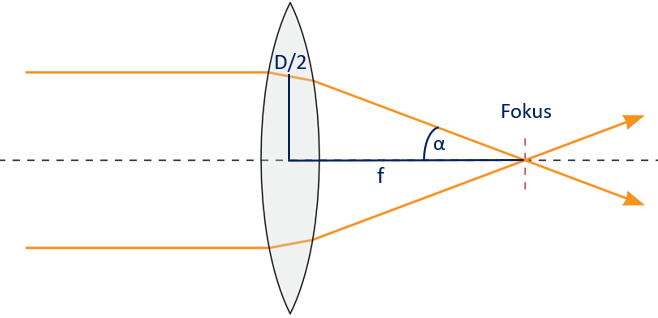
\includegraphics[width=0.57\textwidth]{Linse.png} }}
    \qquad
    \subfloat[\centering Fokusdurchmesser]{{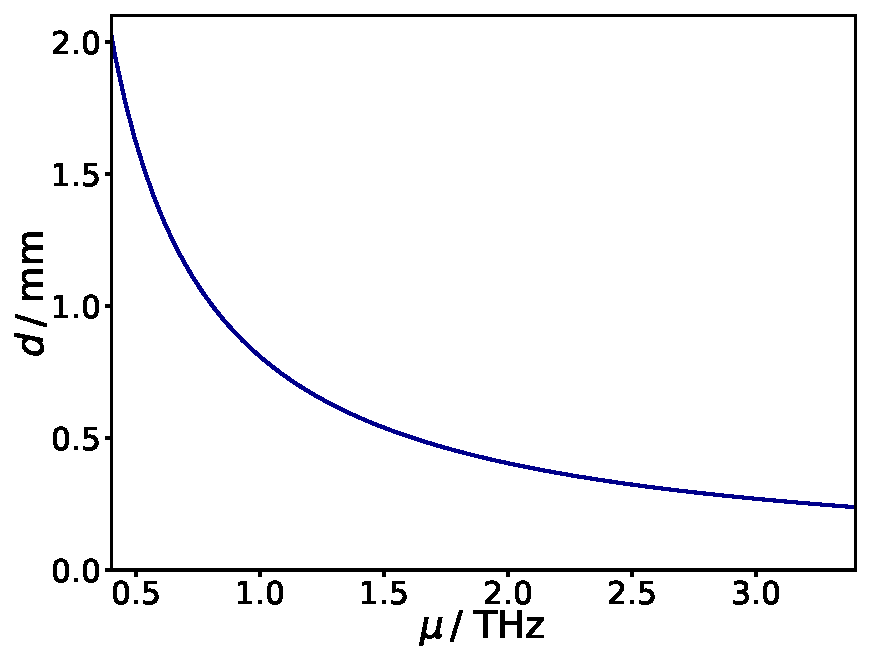
\includegraphics[width=0.35\textwidth]{fokus.pdf} }}
    \caption{\label{fig:abbe}a) Schematische Darstellung der Fokussierung eines Lichtstrahls des Durchmessers $D$
    durch eine Sammellinse der Brennweite $f$. Der halbe Öffnungswinkel $\alpha$ lässt sich 
    über geometrische Überlegungen berechnen. Graphikvorlage entnommen aus Ref.~\cite{Bild1}. \\
    b) Fokusdurchmesser als Funktion der Lichtfrequenz für die betrachteten Linsenparameter im 
    Bereich der THz-Strahlungsfrequenz.}
\end{figure}\FloatBarrier
Der Sinus dieses Winkels lässt sich über die Trigonometrischen Gleichungen berechnen, womit 
eine Bestimmungsgleichung des theoretischen Fokusdurchmessers folgt, die reziprok proportional zur 
Frequenz des Lichtstrahls ist
\begin{align}
    n\sin(\alpha) &= \frac{\text{Gegenkathete}}{\text{Hypothenuse}} = \frac{D/2}{\sqrt{(D/2)^{2} + f^{2}}} \\
    \Rightarrow\Aboxed{d &= \frac{c}{\nu}\frac{\sqrt{(D/2)^{2} + f^{2}}}{D/2}}.
\end{align}
Hieraus erkennt man, dass die Fokussierung mit steigender Frequenz besser wird.
Folgende Werte gelten für die fokussierten Strahlendruchmesser
\begin{equation}
    \fbox{$d_{\nu=0,5\,\si{THz}} \approx 1,6\,\si{mm}\hspace{1cm}d_{\nu=3\,\si{THz}} \approx 0,3\,\si{mm}
    \hspace{1cm}d_{\lambda=1550\,\si{nm}} \approx 4,2\,\si{\mu m}$}.
\end{equation}
Die Frequenzabhängigkeit des Fokusdurchmessers ist für die betrachteten Linsenparameter in Abb.~\ref{fig:abbe}
dargestellt.

    \newpage
    \section{\label{sec:aufbau}Aufbau}
Der am Versuchstag verwendete Aufbau ist schematisch in Abb.~\ref{fig:aufbau} dargestellt. 
\begin{figure}[h!]
    \centering
    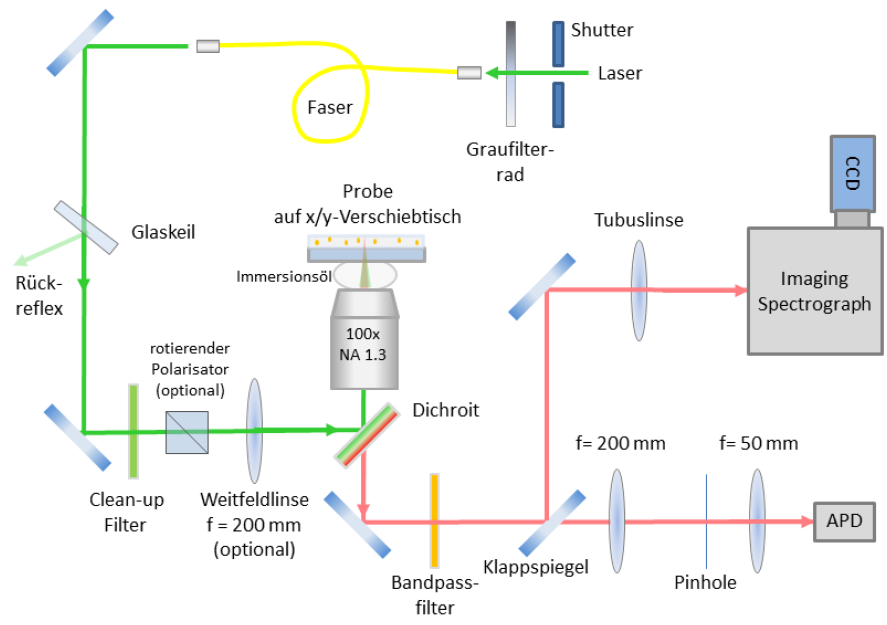
\includegraphics[width=0.7\textwidth]{Versuchsaufbau.png}
    \caption{\label{fig:aufbau}Skizze des Versuchsaufbaus zur Detektion einzelner Moleküle. 
    Die Funktionsweise der einzelnen Komponenten und optionale Variationen sind im Haupttext beschrieben.
    Die Grafik wurde der Anleitung \cite{Anleitung} entnommen.
    Der konfokale Aufbau mit dem Pinhole und der APD (Avalanche Photodiode)
    wird am Versuchstag nicht verwendet.}
\end{figure} \FloatBarrier
Zunächst wird das Laserlicht eines Diodenlasers ($\lambda = 510\,\si{nm}$) über eine Glasfaser 
in den Strahlengang eingekoppelt und über einen Faserpolarisator (nicht eingezeichnet) zirkular polarisert. 
Ein Shutter vor dem Laser ermöglicht es während einer Messpause die Anregungszeit der
Probe zu reduzieren, um das Ausbleichen der Moleküle zu vermeiden. Zudem kann die Anregungsleistung über Graufilterrad 
eingestellt werden. Über Spiegel wird der Strahl auf den dichroitischen Filter geleitet, welcher für verschiedene 
Wellenlänge reflektierend oder transmittierend wirkt (vgl.~Abschnitt \ref{subsec:FZV6}). Der Filter ist so gewählt,
dass das energiereichere Anregungslicht in das Mikroskopobjektiv reflektiert wird, wo es auf die Probe 
fokussiert, welche auf einem verschiebbaren Tisch befestigt ist. Das von der Probe emittierte energieärmere 
Fluoreszenzlicht wird vom Filter durchgelassen. 
Der Clean-up Filter im vorderen Strahlengang unterdrückt unerwünschte Störsignale der optischen Bauteile, während 
der Glaskeil als Kontrollelement für die Fokussierung der Probe genutzt wird. \\
Nach Transmission durch den dichroitischen Filter wird der Strahl über Spiegel in den Spektrographen geleitet. 
Ein Bandpassfilter säubert das Fluoreszenzlicht nochmals von restlichem Anregungslicht, um das Signal-Rausch-Verhältnis 
zu optimieren. Durch die Tubuslinse im Strahlengang ist das Mikroskop vollständig und das vergrößerte Bild 
gelangt in den Spektrographen, welcher wahlweise ein Gitter (150 Linien/mm) oder einen Spiegel in den Strahlengang 
beifügt. Das Signal wird über eine Einzelphotonen-empfindliche CCD Kamera gemessen, die für den Versuch mit 
2x2-Binning betrieben wird (vgl.~Abschnitt \ref{subsec:FZV10}). \\ 
Der Versuchsaufbau lässt sich durch optionale Bauteile variieren. 
Wird die Weitfeldlinse in den Strahlengang geklappt, so kann die Probe großflächig angeregt werden und das 
Signal über den Spektrographen im Spiegelmodus auf die CCD-Kamera geleitet werden. Hierzu muss der 
Spalt weit geöffnet sein. Will man die Spektren der einzelnen Moleküle aufnehmen, so muss das Gitter 
im Spektrographen eingestellt. Außerdem wird die Weitfeldlinse entfernt, wodurch 
sich das angeregte Probenvolumen verkleinert. \\ 
Für die Polarisationsabhängige Messung kann ein rotierender Polarisator eingebracht werden. Zudem lässt sich 
die Anregungsleistung über ein einklappbares Powermeter (nicht eingezeichnet) bestimmen, welches 
vor der Weitfeldlinse im Strahlengang platziert werden kann. \\
Die Durchführungsschritte der einzelnen Versuchsteile, sowie die Präsentationen und Analysen der 
Ergebnisse werden im nächsten Abschnitt beschrieben. \\



    \newpage
    \section{\label{sec:auswertung}Ergebnisse und Diskussion}
\subsection{Röntgenstrahlbeugung: Die Kristallstruktur von Kochsalz (NaCl)} 

\subsection{Bestimmen und Fitten der Peaks}
In diesem Versuchsteil wurde ein Pulverdiffaktogramm von Kochsalz (NaCl) aufgenommen. Die so aufgenommenen Daten sollen nun insbesondere anhand der Peaks analysiert werden. Zuerst werden die Peaks "händisch" mit dem Auge identifiziert. Zudem werden die Peaks mithilfe der Software Jana2020 \footnote[number]{Institute of Physics,Department of StructureAnalysis, Cukrovarnicka 10, 16253 Praha 6, Czech Republic} mit einer Pseudo-Voigt-Funktion gefittet. Als Anfangsfitwert für den Gitterparameter wird hierbei der Literaturwert $a = \SI[options]{5,64}[pre-unit]{\angstrom}$ verwendet. Peaknummer, händisch bestimme Peaklage $2\theta_{[Auge]}$, gefittet Peaklage $2\theta_{[Fit]}$ sowie die Halbwertsbreite sind in Tabelle \ref{tab:peaks} dargestellt.


\begin{table}[h]\label{tab:peaks}
    \centering
     \begin{tabular}{|c|c|c|c|} 
     \hline
     Peak-Nr. & $2\theta_{[Auge]}$ & $2\theta_{[Fit]}$ & FWHM in ° \\ [0.5ex] 
     \hline\hline
     1 & \num[options]{27,46(0,05)} & \num[options]{27,518(0,005)} & \num[options]{0,308(0,005)} \\ 
     2 & \num[options]{31,85(0,03)} & \num[options]{31,881(0,005)} & \num[options]{0,311(0,005)} \\
     3 & \num[options]{45,78(0,05)} & \num[options]{45,709(0,005)} & \num[options]{0,324(0,005)} \\
     4 & \num[options]{54,18(0,03)} & / & / \\
     5 & \num[options]{56,85(0,03)} & \num[options]{56,808(0,005)} & \num[options]{0,338(0,005)} \\ 
     6 & \num[options]{66,66(0,03)} & \num[options]{66,634(0,005)} & \num[options]{0,355(0,005)} \\
     7 & \num[options]{73,75(0,05)} & / & / \\
     8 & \num[options]{75,43(0,03)} & \num[options]{75,774(0,005)} & \num[options]{0,375(0,005)} \\
     9 & \num[options]{84,58(0,03)} & \num[options]{84,554(0,005)} & \num[options]{0,399(0,005)} \\
     10 & \num[options]{89,52(0,05)} & / & / \\
     11 & \num[options]{101,86(0,03)} & \num[options]{101,934(0,005)} & \num[options]{0,467(0,005)} \\
     12 & \num[options]{108,51(0,05)} & / & / \\
     13 & \num[options]{110,80(0,03)} & \num[options]{110,955(0,005)} & \num[options]{0,517(0,005)} \\  [1ex] 
     \hline
     \end{tabular}
\end{table}

Hierbei wird ersichtlich, dass nicht für alle Peaks ein sinnvoller Fit möglich war. Ebenso war die integrierte Intensität mit der Software nicht möglich und wird daher weggelassen. 

\subsection{Gitterparameter und Diskussion}

Nun soll für jeden erfolgreich gefitteten Peak der zugehörige Netzabstand berechnet werden. Hierbei gilt unter Annahme eines kubischen Kristallgitters:
\begin{equation}\label{eq:netzabstand}
    \frac{1}{d^2_{hkl}} = \frac{h^2 + k^2 + l^2}{a^2}
\end{equation}
mit $h, k, l$ den Millerschen Indizes und $a$ dem Gitterparameter. Mithilfe der Braggschen Beugungsbedingung
\begin{equation}
    2d\sin(\theta) = n\lambda
\end{equation}

mit $n = 1$ der Beugungsordnung und $\lambda = \SI[options]{1,5406}{\angstrom}$ der Wellenlänge der Röntgenstrahlung, kann der Gitterparameter berechnet werden:

\begin{equation}
    \sin^2(\theta) = \frac{\lambda^2}{4a^2} \cdot (h^2 + k^2 + l^2)
\end{equation}

Die Ergebnisse für den Netzabstand $d_{hkl}$, deren quadrierten Sinus des Beugungswinkels, die Konstante $\nicefrac[fontcmd]{\lambda^2}{4a^2}$ und den Gitterparameter $a$ sind in Tabelle \ref{tab:gitter} dargestellt. Ebenso werden die Millerschen Indizes für den jeweiligen Peak angegeben.

\begin{table}[h]\label{tab:gitter}
    \centering
     \begin{tabular}{|c|c|c|c|c|c|c|c|} 
     \hline
     Peak-Nr. & $2\theta_{[Fit]}$ & $d/\si[options]{\angstrom}$ & $\sin^2(\theta)$ & $\frac[fontcmd]{\lambda^2}{4a^2}$ & $(h^2+k^2+l^2)$ & $a/\si[options]{\angstrom}$ &  $h k l $ \\ [0.5ex] 
     \hline\hline
     1 & \num[options]{27,518(0,005)} & 3,2387 & 0,056568 & 0,018856 & 3 & 5,6096 & 1 1 1 \\
     2 & \num[options]{31,881(0,005)} & 2,8048 & 0,075424 & 0,018856 & 4 & 5,6096 & 2 0 0 \\
     3 & \num[options]{45,709(0,005)} & 1.9833 & 0.150849 & 0,018856 & 8 & 5,6096 & 2 2 0 \\
     5 & \num[options]{56,808(0,005)} & 1.6194 & 0.226273 & 0,018856 & 12 & 5,6096 & 2 2 2 \\ 
     6 & \num[options]{66,634(0,005)} & 1.4024 & 0.301698 & 0,018856 & 16 &  5,6096 & 0 0 4\\
     8 & \num[options]{75,774(0,005)} & 1.2543 & 0.377122 & 0,018856 & 20 &  5,6096 & 2 0 4\\
     9 & \num[options]{84,554(0,005)} & 1.1451  &  0.452546 & 0,018856 & 24 &  5,6096 & 2 2 4\\
     11 & \num[options]{101,934(0,005)} & 0.9916 & 0.603395 & 0,018856 & 32 &  5,6096 & 4 0 4\\
     13 & \num[options]{110,955(0,005)} & 0.9349 & 0.678820 & 0,018856 & 36 &  5,6096 & 4 2 4\\ [1ex] 
     \hline
     \end{tabular}
\end{table}

Wie man sieht, ist der Gitterparameter $a$ für alle Peaks gleich. Dies liegt natürlich auch an der Natur des Fits, welcher den Gitterparamter berechnet, für den die Abweichungen der gemessenen Werte von den theoretisch bewerteten Werten minimal sind. Daher ist die Mittelwertbildung hier überflüssig, eher kann man direkt den berechneten Wert für $a$ nehmen, den Jana2020 berechnet. Hiermit ergibt sich:

\begin{equation}
    a = \SI[options]{5,6096(0,0005)}{\angstrom}
\end{equation}

Hiermit können nun auch die Netzabstände mithilfe Gl.~\ref{eq:netzabstand} für die Peaks berechnet werden, bei denen kein Fit möglich war. Die Ergebnisse hierfür sind in Tabelle \ref{tab:nonfitval} dargestellt.

\begin{table}[h]\label{tab:nonfitval}
    \centering
     \begin{tabular}{|c|c|c|c|c|c|} 
     \hline
     Peak-Nr. & $2\theta_{[Auge]}$ & $d/\si[options]{\angstrom}$ & $\sin^2(\theta)$ & $(h^2+k^2+l^2)$&  $h k l $ \\ [0.5ex] 
     \hline\hline
     4 & \num[options]{54,18(0,03)} & 1.6914 & 0.207380 & 11 & 1 1 3 \\
     7 & \num[options]{73,75(0,05)} & 1.2869 & 0.360085 & 19 & 3 1 3\\
     10 & \num[options]{89,52(0,05)} &  & 1.0796 & 0.495811 & 27 & 3 3 3 \\
     12 & \num[options]{108,51(0,05)} & 0.9482 & 0.658735 & 35 & 3 1 5 \\
     \hline
     \end{tabular}
\end{table}
\subsubsection{Systematische Auslöschungen und mögliche Raumgruppen}
Die Anzahl der Formeleinheiten $Z$ pro Elementarzelle lässt sich mit der Gleichung aus der Anleitung folgendermaßen bestimmen~\cite[]{Anleitung}:
\begin{equation}\label{eq:formeleinheit}
    Z = \frac{N_A \cdot \rho_x \cdot V_{EZ}}{M_M} \approx 4
\end{equation}
Es ist $N_A$ die Avogadro-Konstante, $\rho_x = \SI{2,17}[]{\gram \per \cubic \centi\metre}$ die Dichte von Kochsalz, $V_{EZ} = a^3$ das Volumen der Elementarzelle und $M_M = \SI{58,44}[]{\gram \per \mol}$ die molare Masse des Materials~\cite[]{Anleitung}.\\
Jetzt werden die gefundenen und indizierten Peaks aus Tab.~\ref{tab:gitter} und Tab.~\ref{tab:gitter2} den Reflexklassen $hkl, 0kl, hhl $ und $00l$ in Tab.~\ref{tab:zuordnung} zugeordnet. Die angegebene Bedingung ist hierbei immer geradezahlig, d.h. $h+k = 2n$ oder $l = 2n$.

\begin{table}[h!]
    \centering
     \begin{tabular}{|c|c|c|c|} 
     \hline
     Peak-Nr. &  $h k l$ & Klasse & Bedingung\\ [0.5ex] 
     \hline\hline
     1 & (1 1 1) & $hkl$ &  $h+k, h+l, k+l$ \\
     2 & (2 0 0) & $00l$ & $l$\\
     3 & (2 2 0) & $hhl$ &  $h+l, l, h$\\
     4 & (1 1 3) & $hhl$ & $h+l, l, h$\\
     5 & (2 2 2) & $hhl$ & $h+l, l, h$\\
     6 & (0 0 4) & $00l$ & $l$\\
     7 & (3 1 3)& $hhl$ & $h+l, l, h$\\
     8 & (2 0 4) & $0kl$ & $k, l$\\
     9 & (2 2 4) & $hhl$ & $h+l, l, h$\\
     10 & (3 3 3) & $hhl$ & $h+l, l, h$\\
     11 & (4 0 4) & $hhl$ & $h+l, l, h$\\
     12 & (3 1 5) & $hkl$ & $h+k, h+l, k+l$\\
     13 & (4 2 4) & $hhl$ & $h+l, l, h$\\  [1ex]
     \hline
    
     \end{tabular}
     \caption[short]{Zuordnung der Peaks zu den Reflexklassen.}
     \label{tab:zuordnung}
\end{table}

Laut den Angaben aus der Tabelle und aus dem Skript ist die einzig mögliche Raumgruppe für Kochsalz die $Fm\overline{3}m$-Gruppe. NaCl ist also frächenzentriert und hat damit 4 Gitterpunkte in einer Elementarzelle (jeweils $\nicefrac[]{1}{8}$ an den Ecken und jeweils $\nicefrac{1}{2}$ an den Flächen), was mit dem berechneten Wert für $Z$ aus Gl.~\ref{eq:formeleinheit} übereinstimmt.\\
\subsubsection{Kristallstruktur und Sturkturfaktor}
\label{sec:kristallstruktur}

In der Praktikumsanleitung gibt es zwei verschiedene Strukturmodelle A und B, die anhand der spektralen Intensitäten bewertet und auf ihre Richtigkeit überprüft werden sollen.
In Strukturmodell A liegt das Chloratom auf $(x,y,z) = (\frac{1}{2}, \frac{1}{2}, \frac{1}{2})$, in Strukturmodell B auf $(x,y,z) = (\frac{1}{4},\frac{1}{4},\frac{1}{4},)$. Das Natriumatom liegt in beiden Modellen auf $(x,y,z) = (0,0,0)$. Für beide Modelle gilt für den jeweiligen Besetzungsfaktor $n_j = 1$. Die Intensität für den Peak $hkl$ ist gegeben durch
\begin{equation}
    I_{hkl} \propto K \cdot A \cdot L \cdot P \cdot E \cdot H \cdot T \cdot \left|F_{hkl}\right|^2
\end{equation}
mit dem Lorentzfaktor $L(\theta)$, dem Polarisationsfaktor $P(\theta)$, dem Absorptionsfaktor $A(\theta)$, dem Strukturfaktor $\left|F_{hkl}\right|^2$, dem Temperaturfaktor $T(\theta)$, dem Extiktionsfaktor $E(\theta)$ und einem Skalierungsfaktor $K$. Für die Faktoren gilt:
\begin{equation}
    L (\theta)= \frac{1}{\sin(\theta) \cos(\theta)}
\end{equation}
\begin{equation}
    P (\theta) = \frac{1 + \cos^2(2\theta)}{2}
\end{equation}
\begin{equation}
    \left|F_{hkl}\right|^2 = F_{hkl} \cdot F_{hkl}^*
\end{equation}
mit der Strukturamplitude $F_{hkl}$
\begin{equation}
    F_{hkl} = \sum_{j = 1}^{N} \left[n_j f_j \cdot \exp \{2\pi i \left(hx_j+ky_j+lz_j\right)\}\right]
\end{equation}
und dem Atomformfaktor $f\left(\frac{\sin\left(\Theta\right)}{\lambda}\right)$
\begin{equation}
    f\left(\frac{\sin\left(\Theta\right)}{\lambda}\right) = \sum_{i=1}^4 \left[a_i \cdot \exp\left(-b_i \cdot \left(\frac{\sin(\Theta)}{\lambda}\right)^2\right)\right] + c
\end{equation}
Alle diese Größen werden nun für die gefitteten Peaks aus Kapitel~\ref{sec:peaks} berechnet. Die Ergebnisse sind in Tabelle~\ref{tab:ergebnisse} dargestellt.
\begin{table}[h!]
    \centering
\begin{tabular}{|c|c|c|c|c|c|c|c|c|c|c|c|c|}
    \hline
   Peak-Nr. & $2\Theta_[Fit]$& $hkl$ & $L$ & $P$ & $H$ & $f_{Na}$ & $f_{Cl}$ & $F_{hkl, A}$& $F_{hkl, B}$ & $\left|F_A^2\right|$ & $\left|F_A^2\right|$ \\ [0.5ex]
   \hline\hline
   1 & 27.518 & 1 1 1&4.33 & 0.89 & 1 & 6.78 & 9.45 & -2.67+0.00i & 6.78-9.45i & 7.13 & 135.41 \\
   2 & 31.881 &2 0 0& 3.79 & 0.86 & 3 & 6.11 & 8.73 & 14.84-0.00i & -2.63+0.00i & 220.21 & 6.90 \\
   3 & 45.709 &2 2 0& 2.79 & 0.74 & 3 & 4.34 & 7.35 & 11.69-0.00i & 11.69-0.00i & 136.69 & 136.69 \\
   5 & 56.808 &2 2 2& 2.39 & 0.65 & 1 & 3.40 & 6.60 & 10.00-0.00i & -3.20+0.00i & 99.92 & 10.23 \\
   6 & 66.634 &0 0 4& 2.18 & 0.58 & 3 & 2.84 & 6.01 & 8.85-0.00i & 8.85-0.00i & 78.30 & 78.30 \\
   8 & 75.774 &2 0 4& 2.06 & 0.53 & 6 & 2.48 & 5.53 & 8.01-0.00i & -3.04+0.00i & 64.09 & 9.27 \\
   9 & 84.554 &2 2 4& 2.01 & 0.50 & 3 & 2.24 & 5.12 & 7.36-0.00i & 7.36-0.00i & 54.20 & 54.20 \\
   11 &101.934 &4 0 4& 2.04 & 0.52 & 3 & 1.96 & 4.52 & 6.47-0.00i & 6.47-0.00i & 41.91 & 41.91 \\
   13 & 110.955 &4 2 4& 2.14 & 0.56 & 3 & 1.88 & 4.30 & 6.18-0.00i & -2.43+0.00i & 38.15 & 5.89 \\ [1ex]
   \hline
   \end{tabular}    
   \caption[short]{Ergebnisse der Berechnung der Strukturfaktoren für die gefitteten Peaks.}
   \label{tab:ergebnisse}
\end{table}

Für die Berechnung der Intensitäten werden nun $A$, $E$ und $T$ auf 1 gesetzt und die Intensitäten für beide Modelle auf die (2 0 0) Intensität normiert. Die Ergebnisse sind in Tabelle~\ref{tab:ergebnisse2} dargestellt.

\begin{table}[h!]
    \centering
    \begin{tabular}{|c|c|c|c|c|c|}
        \hline
        Peak-Nr. & $hkl$&$I_A$ & $I_B$ & $I_{norm,A}$ & $I_{norm,B}$ \\ [0.5ex]
        \hline\hline
       1 & 1 1 1 &27.6 & 523.6 & 0.01 & 7.77 \\
       2 & 2 0 0&2152.8 & 67.4 & 1.00 & 1.00 \\
       3 & 2 2 0&852.2 & 852.2 & 0.40 & 12.64 \\
       5 & 2 2 2&155.2 & 15.9 & 0.07 & 0.24 \\
       6 & 0 0 4&296.1 & 296.1 & 0.14 & 4.39 \\
       8 & 2 0 4&420.7 & 60.8 & 0.20 & 0.90 \\
       9 & 2 2 4&164.8 & 164.8 & 0.08 & 2.44 \\
       11 & 4 0 4&134.0 & 134.0 & 0.06 & 1.99 \\
       13 & 4 2 4&138.2 & 21.3 & 0.06 & 0.32 \\ [1ex]
       \hline
       \end{tabular}
        \caption[short]{Ergebnisse der Berechnung der Intensitäten für die gefitteten Peaks.}
        \label{tab:ergebnisse2}
\end{table}

Wie bereits erwähnt, war eine Integration der gemessenen Intensitäten sehr komlex, was eine quantitave Aussage über die Richtigkeit der Modelle nicht möglich macht. Rein qualitativ anhand der Höhe der Intensitäten, sichtbar in Abb.~\ref{fig:geglättet}, insbesondere verglichen mit dem zweiten Normierungspeak (2 0 0), lässt sich sagen, dass Modell A deutlich besser zu den Daten passt. Dies ist bereits am ersten Peak erkennbar: Im gemessenen Spektrum ist dieser deutlich kleiner als der Maximalpeak, auf den hier normiert wurde. Dies deckt sich mit den Daten aus Modell A, nicht jedoch mit Modell B, laut dem Peak 1 über 7 mal so hoch wie Peak 2 wäre. Auch die anderen Peaks zeigen eine ähnliche Tendenz. Dadurch lässt sich also klar sagen, dass das Natriumatom bei $(x,y,z) = (0,0,0)$ und das Chloratom bei $(x,y,z) = (\frac{1}{2}, \frac{1}{2}, \frac{1}{2})$ sitzt.
\subsubsection{Gerätefunktion}
\label{sec:geraetefunktion}

Ein gemessenes Spektrum kann als Faltung von Geräte- und Probenfunktion interpretiert werden. 
Aufgrund der hohen Kristallinität von Kochsalz kann hier jedoch der Anteil der Probe an der Halbwertsbreite der Peaks vernachlässigt werden. Daraus folgt, dass die Halbwertsbreitenfunktion in etwa der Gerätefunktion entspricht. Die Halbwertsbreitenfunktion ist gegeben durch~\cite[]{Anleitung}:
\begin{equation}
    FWHM(\Theta) = \sqrt{U \cdot \tan^2(\Theta) + V \cdot \tan(\Theta) + W}
\end{equation}
Mithilfe von scipy.optimize.curve\_fit können nun die Parameter $U, V, W$ bestimmt werden. Die Messwerte werden aus Tabelle~\ref{tab:peaks} übernommen. Für die Fitparameter ergibt sich:
\begin{equation*}
    U = \num{84,3(0,5)e-3}, \qquad V = \num{-0,5(0,8)e-3}, \qquad W = \num{90,0(0,3)e-3}
\end{equation*}
Messwerte und Fit sind in Abbildung~\ref{fig:geraetefunktion} dargestellt.

\begin{figure}[hbt!]
    \centering
    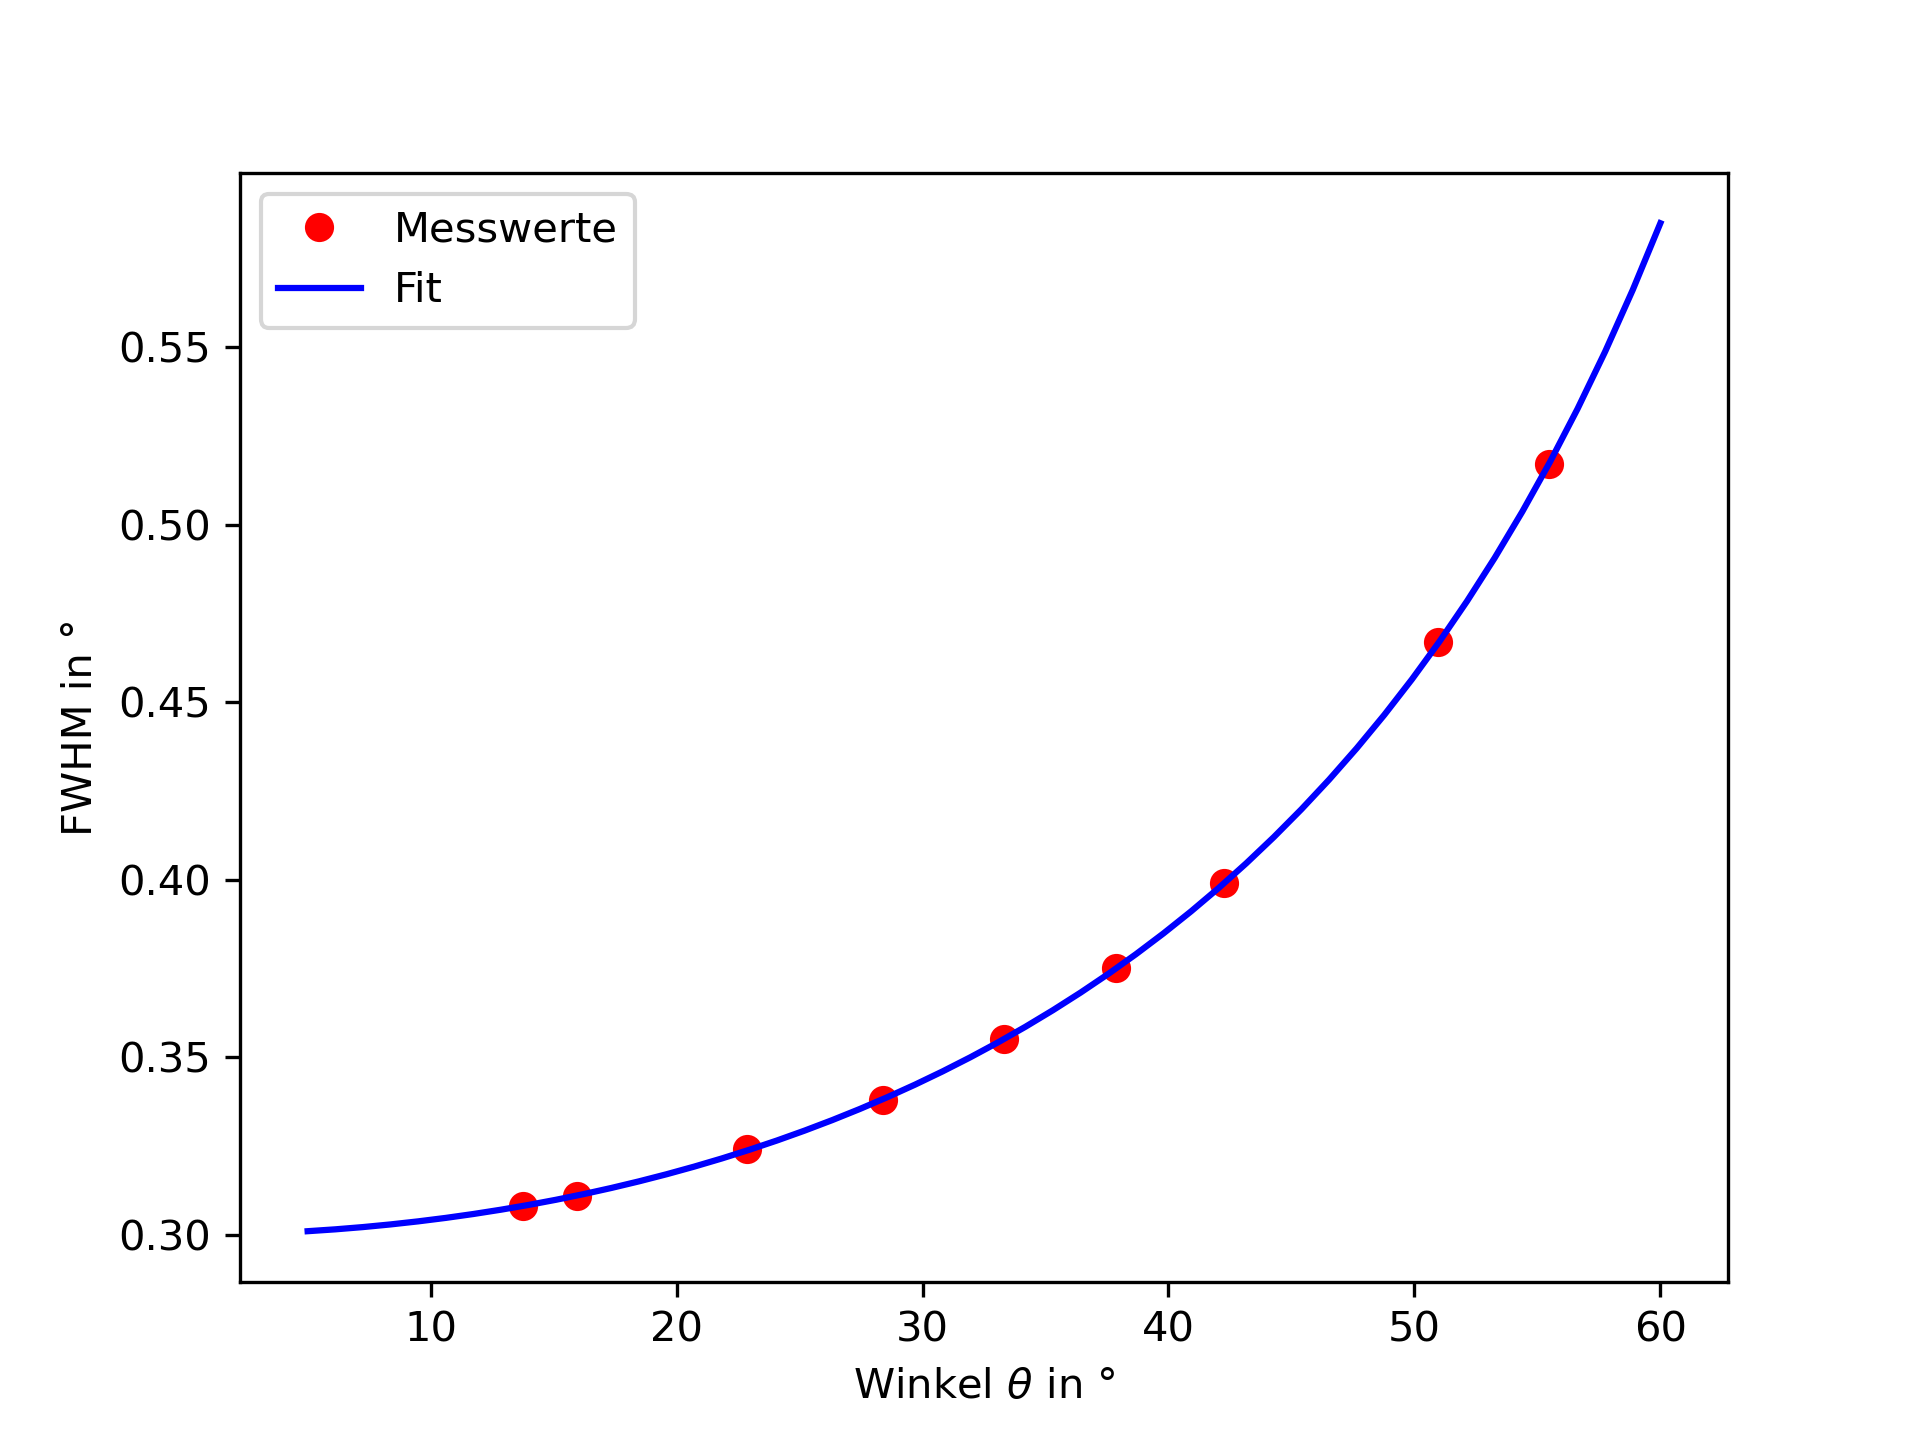
\includegraphics[width=0.7\textwidth]{fwhm_fit.png}
    \caption{Halbwertsbreite als Funktion des Streuwinkels mit den Messwerten in Rot und dem Fit in blau.}
    \label{fig:geraetefunktion}
\end{figure}

Der Fit passt sehr gut zu den gemessenen Halbwertsbreiten, in der hier gemessenen Gerätefunktion lässt sich jedoch kein wirkliches Minimum feststellen. Ein Minimum stände hierbei für den Punkt der geringsten Streuung am Detektor, was für die genauesten Messwerte stände.


\subsubsection{Beurteilung der Messung}
Insgesamt können wir mit der Messung zufrieden sein. Die Peaks sind gut zu erkennen und die berechnete Gitterkonstante liegt nah am Literaturwert. Die Peaks sind jedoch nicht so scharf wie in der Theorie, was auf eine gewisse Unschärfe des Detektors zurückzuführen ist. Auch der Fit der Jana2020 Software hat gut funktioniert. Der Großteil der erkennbaren Peaks konnte gut gefittet werden, was ebenso auf eine funktionerende Messung schließen lässt. Mit den gewonnenen Werten konnte auch ein gutes Modell für den Aufbau des NaCl-Kristalls bestätigt werden.\\
Bei zukünftigen Messungen könnte durch eine Verlängerung der Messdauer leicht die Genauigkeit bzw. das Signal-Rausch-Verhältnis erhöht werden. Auch eine bessere Justierung des Detektors könnte die Messung verbessern. Für die Erfassung von mehr Peaks könnte ebenso der Winkelbereich vergrößert werden.
\clearpage


    \newpage
    \section{\label{sec:fazit}Fazit}
In diesem Versuch haben wir uns sowohl mit Röntgenabsorption als auch mit Röntgenbeugunt beschäftigt. Zum Anfang haben wir nach langer Kalibrierung Absorptionsspektren sowohl mit also auch ohne Absorberfolie aufgenomomen, um einen Zusammenhang zwischen Winkel und Wellenlänge zu finden. Hier konnten wir schön die zuvor nur theoretisch bekannten Absoprtionskanten entdecken. Dieses neu gewonnene Wissen konnten wir daraufhin direkt zur Identifizierung eines Metalls nutzen, was sehr spannend war.\\
Im zweiten Versuchsteil haben wir dann versucht, anhand von Röntgenbeugung mehr über die Kristallstruktur von Kochsalz zu erfahren. Anhand eines aufgenommenen Diffraktogramms konnten wir die verschiedenen Peaks finden, fitten und damit die Gitterkonstante bestimmen. Ebenso haben wir uns verschiedene Modelle für die Anordnung der Atome in der Elementarzelle angeschaut und konnten nur anhand der Peakintensitäten das richtige Modell herausfinden. Da die Kristallstruktur von Kochsalz bereits in der Schule gelehrt wird, war es sehr spannend, dies endlich für uns selber herauszufinden. \\
Insgesamt hat der Versuch uns einen guten Einblick in die Arbeit eines Kristallografen geben können und hat definitiv geholfen, ein vertieftes Verständnis für die Röntgenbeugung zu entwickeln, welches zuvor nur aus Festkörperphysikvorlesungen bekannt war. Auch wenn nicht alles auf Anhieb geklappt hat, war der Versuch sehr lehrreich und informativ, hat sich gelohnt und uns insbesondere bei der Auswertung Freude bereitet.  
    \newpage
    % \appendix
    % \numberwithin{equation}{section}
    % \input{Input/}
    % \newpage
    \printbibliography
\end{document}
